% !TEX root = memoire.tex
\chapter{Préliminaires}

Dans ce premier chapitre nous définissons les polyominos et nous introduisons quelques concepts de base s'y rattachants.

\section{Les polyominos}

\begin{definition}
Une \emph{cellule} est un carré unitaire $[x,x+1] \times [y,y+1] \subseteq \R^2$. Ses côtés sont appelés \emph{arêtes}.
\end{definition}

\begin{definition*}
Deux cellules sont dites \emph{4-adjacentes} (resp. \emph{8-adjacentes}) si elles partagent au moins une arête (resp. un sommet).
\end{definition*}

Une définition justifiée par le fait qu'une cellule possède un maximum de $4$ ou $8$ voisins selon le type de connexité.

\begin{definition*}
Un ensemble de cellules est \emph{connexe} si toute paire de cellules est reliée par une suite de cellules adjacentes.
\end{definition*}

\begin{figure}[h]
\centering
\begin{tikzpicture}
\squarepath[orange]{(0,1)}{701}
\pas{0.5,1.5}{1.5,0.5};
\pas{1.5,0.5}{2.5,0.5};
\pas{2.5,0.5}{3.5,1.5};
\expandboundingbox
\end{tikzpicture}
\caption[Un chemin]{Un chemin dans un ensemble de cellules $8$-connexe.}
\end{figure}

Nous pouvons maintenant proposer une première définition du polyomino :

\begin{definition}
Un \emph{polyomino} est un ensemble de cellules $4$-connexe.
\end{definition}

\begin{figure}
\begin{subfigure}[b]{.5\linewidth}
\centering
\scalebox{.5}{
\polyomino[blue]{020}

\polyomino[green]{022446} 

\polyomino[red]{000224466}
}
\caption{Des polyominos}
\end{subfigure}
\begin{subfigure}[b]{.5\linewidth}
\centering
\scalebox{.5}{

\begin{tikzpicture}
\squarepath[orange]{(0,0)}{20}
\squarepath[orange]{(1,-1)}{02}
\expandboundingbox
\end{tikzpicture}

\begin{tikzpicture}
\squarepath[violet]{(0,0)}{000022224444666}
\squarepath[violet]{(2,2)}{{}}
\expandboundingbox
\end{tikzpicture}


\includegraphics[scale=.3]{dipsy}
}
\caption{Pas des polyominos}
\end{subfigure}
\caption{Exemples de polyominos}\label{fig:exemples-de-polyominos}
\end{figure}

On remarque à la figure \ref{fig:exemples-de-polyominos} que cette définition implique l'existence de polyominos contenant des ``trous''.

\begin{definition}
Soit $P$ un polyomino. Le \emph{contour extérieur} de $P$, $C_e(P)$, est l'ensemble des cellules $4$-connexe à $P$ n'appartenant pas à $P$.
\end{definition}

\begin{definition}
Soit $P$ un polyomino. Son \emph{contour intérieur} $C_i(P)$ est l'intersection entre $P$ et les cellules $4$-connexe à $C_e(P)$.
\end{definition}

Le contour extérieur est connu dans la littérature sous le nom \emph{périmètre de site}. %\cite{Delest:1987aa}.
Pour générer un polyomino, nous générerons son contour défini comme suit \cite{MBM03,Sieben08}  : 

\begin{definition}\label{def:contours}
Le \emph{contour extérieur} d'un polyomino $P$ est l'ensemble $P^+\subseteq\Z^2 \setminus P$ de tous les points $b \in P^+$ qui sont $4$-connexe à au moins un point de $P$. De la même manière, le \emph{contour intérieur} de $P$ est le sous-ensemble $P^-\subseteq P$ de points qui sont $8$-connexes à un point de $\Z^2\setminus P$.
\end{definition}


La figure \ref{fig:contours} illustre le contour intérieur et le contour extérieur d'un polyomino. Il est clair que pour un polyomino donné, ses contours intérieur et extérieur sont uniques.



Quelques propriétés intéressantes :
\renewcommand{\labelitemi}{$\bullet$}
\begin{itemize}
\item $C_e(P) \cap P = \emptyset$
\item $C_i(P) \subseteq P$
\item Pour tout $c \in C_e(P)$, il existe un $t \in P$ tel que $c$ et $t$ sont adjacentes par les côtés.
\end{itemize}




\begin{figure}
\centering
\shorthandoff{:}
\begin{tikzpicture}[scale=0.5]
\draw[color=black!20] (-1.1,-2.1) grid (10.1,8.1);
\squarepath[red]{(0,0)}{000600002022244444444662220000000024444420000};
\savebox{\customwalkbox}{$\circ$}
\custompath{(-0.5,0.5)}{70070000112222233444456445666}
\custompath{(1.5,1.5)}{0070012444444}

\savebox{\customwalkbox}{\large$\bullet$}
\custompath{(0.5,0.5)}{00060000202222242444466444666622200000000}

\squarepath[red]{(11,4.5)}{{}}
\draw (12.5,5) node[right] {Polyomino};

%\draw[tuile] (11,2.5) rectangle ++(1,1);
\draw (11.5,3) node{$\bullet$};
\draw (12.5,3) node[right] {Contour intérieur};

%\draw[draw, black!20] (11,0.5) rectangle ++(1,1);
\draw (11.5,1) node{$\circ$};
\draw (12.5,1) node[right] {Contour extérieur};

\end{tikzpicture}
\caption{Les contours}\label{fig:contours}
\end{figure}


\paragraph{\bf Trous et connexité.}\medskip
On obtient différentes sous-classes de polyominos en ajoutant des contraintes de connectivité. Un polyomino $P$ est \emph{simplement} $4$-connexe (resp. \emph{simplement} $8$-connexe) si son complément $\Z^2 \setminus P$ est également $4$-connexe (resp. $8$-connexe). Par exemple, dans la figure \ref{fig:trous}, le polyomino $P_1$ est simplement $4$-connexe, $P_2$ n'est pas simplement $4$-connexe mais il est simplement $8$-connexe et $P_3$ n'est pas simplement $8$-connexe.
\begin{figure}[h]
\centering
\begin{subfigure}[b]{.2\linewidth}
\centering
\scalebox{.4}{\polyomino[blue]{66020}}
\caption*{$P_1$}
\end{subfigure}
\begin{subfigure}[b]{.2\linewidth}
\centering
\scalebox{.4}{\polyomino[green]{660023}}
\caption*{$P_2$}
\end{subfigure}
\begin{subfigure}[b]{.2\linewidth}
\centering
\scalebox{.4}{\polyomino[red]{66002022446}}
\caption*{$P_3$}
\end{subfigure}
\vspace{-12pt}\caption{Polyominos et trous}
\label{fig:trous}
\end{figure}
\vspace{-12pt}
L'algorithme décrit au chapitre \ref{chapitre-generation} pour la génération exhaustive est assez général pour générer tous ces polyominos. Pour y parvenir, nous devons préciser la notion de \emph{trou}.

\begin{definition}[Trous]\label{def:trous}
Soit $P$ un polyomino. Un \emph{$4$-trou} (resp. \emph{$8$-trou}) de $P$ est un sous-ensemble $4$-connexe (resp. $8$-connexe) maximal et fini de $\Z^2 \setminus P$.
\end{definition}

Ainsi, puisqu'un trou doit être maximal et fini, celui-ci doit être contenu dans un polyomino. Par exemple, dans la figure \ref{fig:trous}, $P_2$ a un $4$-trou, qui dans ce cas est $8$-connexe à une partie infinie de $\Z^2 \setminus P$. Ce n'est donc pas un $8$-trou. Par contre, $P_3$ a un $8$-trou, qui peut aussi être vu comme deux $4$-trous.


\section{Représentations}
Nous avons déjà vu qu'un ensemble de cases connexes par les arêtes est un polyomino.  Il y a plusieurs représentations naturelles qui s'imposent:  graphe de la relation de connectivité, sa réalisation  dans le plan discret $\Z\times\Z$, et  le codage de son contour  par des pas élémentaires. 

\paragraph{\bf Graphe de connexité.}
Parfois l'emplacement précis des cellules n'est pas important, c'est plutôt leur connectivité qui nous intéresse. On construit donc un graphe dont les sommets sont les cellules du polyomino et deux sommets sont reliés par une arête si et seulement si les cellules correspondantes sont $4$-adjacentes.
\begin{figure}[H]
\begin{subfigure}[b]{.5\textwidth}
\centering
\scalebox{0.5}{\polyomino{00204406}}
\end{subfigure}
\begin{subfigure}[b]{.5\textwidth}
\centering
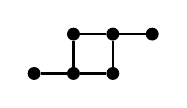
\begin{tikzpicture}[scale=0.5,every node/.style={draw, circle, fill, inner sep=1.5pt}]
\node (a) at (0,0) {};
\node (b) at (1,0) {};
\node (c) at (2,0) {};
\node (d) at (1,1) {};
\node (e) at (2,1) {};
\node (f) at (3,1) {};

\draw[thick] (a) -- (b) -- (c);
\draw[thick] (b) -- (d);
\draw[thick] (c) -- (e);
\draw[thick] (d) -- (e) -- (f);
\end{tikzpicture}
\end{subfigure}
\caption{Un polyomino et son graphe associé}
\end{figure}

\vspace{-24pt}
\paragraph{\bf Sous-ensemble de $\Z^2$.}
Le passage d'un ensemble de tuiles à un ensemble de points à coordonnées entières est naturel. Il suffit de choisir un point canonique sur la tuile, par exemple le plus en bas parmi les plus à gauche. Cette représentation est utilisée entre autre par les physiciens qui nomment ces objets des animaux (\emph{lattice animals} en anglais) \cite{Lubensky79, C3SM52805G} qui surviennent dans des questions reliées à la percolation \cite{KM}.
\begin{figure}[H]
\centering
\shorthandoff{:}
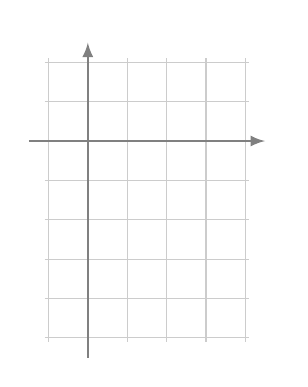
\begin{tikzpicture}[scale=0.5,>=latex,transform shape]
\tuile{0,0};
\tuile{0,1};
\tuile{0,2};
\tuile{0,3};
\tuile{-1,3};
\tuile{0,4};
\tuile{1,0};
\tuile{2,0};
\tuile{0,-1};
\tuile{2,-1};

\begin{scope}[xshift=6.5cm]
\draw[color=black!20] (-2.1, -2.1) grid (3.1,5.1);
\draw[color=black!50, thick, ->] (-1,-2.5) -- (-1,5.5) node [label=above left:$\Z$] {}; 
\draw[color=black!50, thick, ->] (-2.5,3) -- (3.5,3) node [label=below right:$\Z$] {}; 
\point{0,0};
\point{0,1};
\point{0,2};
\point{0,3};
\point{-1,3};
\point{0,4};
\point{1,0};
\point{2,0};
\point{0,-1};
\point{2,-1};
\end{scope}

\end{tikzpicture}
\caption{Un polyomino et son animal}
\end{figure}

Bien que l'utilisation d'éléments de $\Z^2$ donne accès aux outils de la géométrie analytique, le passage du continue au discret reste délicat. Ainsi, même une définition aussi simple que le disque discret $D$ de rayon $r$ centré en $C$ présente certains problèmes
\[
D = \left \{ (x,y) \st {(x-C_x)}^2+{(y-C_y)}^2 \leq r^2, x,y \in \Z\right\}.
\]
Dans \cite{inertia} par exemple, on étudie ces disques et leur comportement lorsque $C$ varie de façon continue dans $\R^2$ (figure \ref{disque-discret}).

\begin{figure}[H]
\centering
\begin{subfigure}{.4\textwidth}
\centering
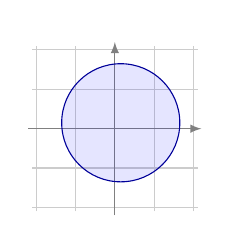
\begin{tikzpicture}[scale=0.5,transform shape,auto]
\shorthandoff{:}
\draw[black!20] (-2.1,-2.1) grid (2.1,2.1);
\draw[black!50, ->, >=latex] (-2.2, 0) -- (2.2, 0) node[label=below right:$\Z$]{};
\draw[black!50, ->, >=latex] (0,-2.2) -- (0, 2.2) node[label=above left:$\Z$]{};
\fill[blue, opacity=.1] (0.15,0.15) circle (1.5);
\draw[blue!60!black] (0.15,0.15) circle (1.5);
\end{tikzpicture}
\caption{Centré en $(0.15,0.15)$}\label{disque-decentre}
\end{subfigure}
\begin{subfigure}{.4\textwidth}
\centering
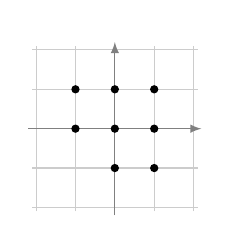
\begin{tikzpicture}[scale=0.5,transform shape,auto]
\shorthandoff{:}
\draw[black!20] (-2.1,-2.1) grid (2.1,2.1);
\draw[black!50, ->, >=latex] (-2.2, 0) -- (2.2, 0) node[label=below right:$\Z$]{};
\draw[black!50, ->, >=latex] (0,-2.2) -- (0, 2.2) node[label=above left:$\Z$]{};
\foreach \p in {(1,0),(1,1),(0,1),(-1,1),(-1,0),(0,-1),(1,-1),(0,0)}
  \fill \p circle (3pt);
\end{tikzpicture}
\caption{Discrétisation de \ref{disque-decentre}}
\end{subfigure}

\centering
\begin{subfigure}{.4\textwidth}
\centering
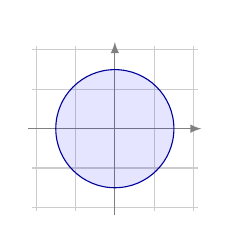
\begin{tikzpicture}[scale=0.5,transform shape,auto]
\shorthandoff{:}
\draw[black!20] (-2.1,-2.1) grid (2.1,2.1);
\draw[black!50, ->, >=latex] (-2.2, 0) -- (2.2, 0) node[label=below right:$\Z$]{};
\draw[black!50, ->, >=latex] (0,-2.2) -- (0, 2.2) node[label=above left:$\Z$]{};
\fill[blue, opacity=.1] (0,0) circle (1.5);
\draw[blue!60!black] (0,0) circle (1.5);
\end{tikzpicture}
\caption{Centré en $(0,0)$}\label{disque-centre}
\end{subfigure}
\begin{subfigure}{.4\textwidth}
\centering
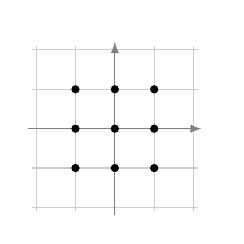
\begin{tikzpicture}[scale=0.5,transform shape,auto]
\shorthandoff{:}
\draw[black!20] (-2.1,-2.1) grid (2.1,2.1);
\draw[black!50, ->, >=latex] (-2.2, 0) -- (2.2, 0) node[label=below right:$\Z$]{};
\draw[black!50, ->, >=latex] (0,-2.2) -- (0, 2.2) node[label=above left:$\Z$]{};
\foreach \p in {(1,0),(1,1),(0,1),(-1,1),(-1,0),(-1,-1),(0,-1),(1,-1),(0,0)}
  \fill \p circle (3pt);
\end{tikzpicture}
\caption{Discrétisation de \ref{disque-centre}}
\end{subfigure}
\caption{Disques de rayon 1.5 et leur équivalent discret.}\label{disque-discret}
\end{figure}


\paragraph{\bf Mot de contour.}

Un \emph{alphabet} est un ensemble fini de symboles. Un \emph{mot} $m$ sur l'alphabet $\mathcal{A}$ est une séquence finie de symboles $a_i \in \mathcal{A}, i \in \N$.
\[
m = a_1 a_1 a_2 \cdots a_{n} 
\]

On note $|m|$ la longueur du mot $m$, et $m_i$ (ou $m[i]$ pour une notation plus près de l'informatique) sa $i^{\rm i\grave{e}me}$ lettre. Le nombre d'occurrences de $\alpha \in \mathcal{A}$ dans $m$ est noté $|m|_\alpha$ et le mot de longueur $0$ est appelé le mot vide qu'on note $\varepsilon$. On remarque que les indices sont entre $1$ et $|m|$ et non entre $0$ et $|m|-1$.

On note $\mathcal{A}^n$ l'ensemble des mots de longueur $n$, et $\mathcal{A}^*$ l'ensemble des mots finis. 

\begin{definition*}
À l'aide de deux mots $a \in \mathcal{A}^m$ et $b \in \mathcal{A}^n$ on obtient par \emph{concaténation}, ou \emph{produit}, le mot $a \cdot b\in \mathcal{A}^{m+n}$, ou simplement $ab$. 
\begin{eqnarray*}
a & = & a_1 a_2 \cdots a_m \\
b & = & b_1 b_2 \cdots b_n \\
ab & = & a_1 a_2 \cdots a_m b_1 b_2 \cdots b_n \\
\end{eqnarray*}
\end{definition*}

%\begin{proposition*}
%$\mathcal{A}^*$ est doté d'une structure de monoïde libre.
%\end{proposition*}

\begin{figure}
\centering
\begin{subfigure}[b]{.25\textwidth}
\centering
\begin{tikzpicture}[scale=.3]
\node[name=O,circle,inner sep=.1cm,fill=black,scale=.4] at (0,0) {};
\node[name=E,draw=none] at (2,0) {$0$};
\node[name=N,draw=none] at (0,2) {$1$};
\node[name=W,draw=none] at (-2,0) {$2$};
\node[name=S,draw=none] at (0,-2) {$3$};
\node[draw=none] at (-3,0) {};
\node[draw=none] at (3,0) {};

\draw[->] (O) to (E);
\draw[->] (O) to (N);
\draw[->] (O) to (W);
\draw[->] (O) to (S);
\end{tikzpicture}
\end{subfigure}
\centering
\begin{subfigure}[b]{.25\textwidth}
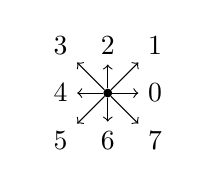
\begin{tikzpicture}[scale=.3]
\node[name=O,circle,inner sep=.1cm,fill=black,scale=.4] at (0,0) {};
\node[name=E,draw=none] at (2,0) {$0$};
\node[name=NE,draw=none] at (2,2) {$1$};
\node[name=N,draw=none] at (0,2) {$2$};
\node[name=NW,draw=none] at (-2,2) {$3$};
\node[name=W,draw=none] at (-2,0) {$4$};
\node[name=SW,draw=none] at (-2,-2) {$5$};
\node[name=S,draw=none] at (0,-2) {$6$};
\node[name=SE,draw=none] at (2,-2) {$7$};
\node[draw=none] at (-3,0) {};
\node[draw=none] at (3,0) {};
\draw[->] (O) to (E);
\draw[->] (O) to (N);
\draw[->] (O) to (W);
\draw[->] (O) to (S);
\draw[->] (O) to (NE);
\draw[->] (O) to (NW);
\draw[->] (O) to (SW);
\draw[->] (O) to (SE);
\end{tikzpicture}
\end{subfigure}
\caption{Directions associées à deux alphabets de Freeman}\label{fig:alphabet-freeman}
\end{figure}


En 1961, Herbert Freeman propose de décrire des chemins en utilisant quatre "pas" élémentaires $(\rightarrow,\uparrow,\leftarrow,\downarrow)\simeq (0,1,2,3)$ associés à des vecteurs tel qu'illustré à la figure \ref{fig:alphabet-freeman} \cite{freeman1}. On note cet alphabet $\mathcal{F}$. On code un polyomino sans trou à l'aide de ces lettres en parcourant son bord, chaque lettre correspondant à un pas unitaire sur le chemin. On verra aux sections \ref{subsection:4-trous} et \ref{subsection:8-trous} comment étendre ce codage aux polyominos avec trou.

L'alphabet de virages décrit quant à lui les changements de direction durant le parcours. On peut passer d'un mot $f$ sur l'alphabet de Freeman à un mot $v$ sur l'alphabet de virages en soustrayant les valeurs consécutives:
\[
v_i = f_{i+1} - f_{i} \mod 4 \quad 1 \leq i \le |f|
\]

Pour cette raison on le nomme aussi alphabet des premières différences. On interprète les valeurs $(0,1,2,3)\simeq ($tout droit, gauche, demi-tour, droite$)$. En nous limitant aux mots de contour, qui ne contiennent pas de demi-tour, l'alphabet des premières différences est donc $\{0,1,3\}$.

Un \emph{$4$-chemin} (respectivement \emph{$8$-chemin}) est un chemin qui n'utilise que des pas unité horizontaux et verticaux (respectivement horizontaux, verticaux et diagonaux) . Si ce chemin est fermé et simple, c'est-à-dire que le point d'origine est visité exactement $2$ fois, tandis que tous les autres points sont visités au maximum une fois, alors ce chemin décrit le contour d'un polyomino sans trou.
\begin{figure}[H]
\begin{subfigure}{.33\linewidth}
\centering
\begin{tikzpicture}
\tuile{0,0};
\tuile{1,0};
\end{tikzpicture}
\end{subfigure}
\begin{subfigure}{.33\linewidth}
\centering
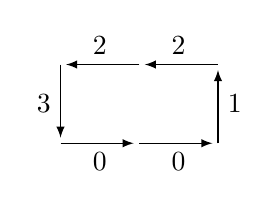
\begin{tikzpicture}[>=latex, auto, pas/.style={->, swap, shorten >=2pt}]
\point{0,0};
\draw[pas] (0,0) to node{$0$} (1,0);
\draw[pas] (1,0) to node{$0$} (2,0);
\draw[pas] (2,0) to node{$1$} (2,1);
\draw[pas] (2,1) to node{$2$} (1,1);
\draw[pas] (1,1) to node{$2$} (0,1);
\draw[pas] (0,1) to node{$3$} (0,0);

%\draw[->, swap, bend right] (0,0) to node{0} (1,0) to node{0} (2,0) to node{2} (2,1) to (1,1) to (0,1) to (0,0);

\end{tikzpicture}
\end{subfigure}\begin{subfigure}{.33\linewidth}\centering \ocr{001223} \end{subfigure}

\caption{Un polyomino, son contour et son mot de contour}
\end{figure}


%\begin{preuve}
%\begin{enumerate}
%\item $\forall a,b \in \A^*, ab \in \A^*.$
%\item $\forall a,b,c \in \A^*, ab(c) = a(bc).$
%\item $\forall a \in A^*, a\varepsilon = \varepsilon a = a.$
%\item $\A$ est une base de $\A^*.$
%\end{enumerate}
%\end{preuve}
